
\subsection{Participants}
The recruitment of 50 L1 Italian L2 English speakers was managed through Prolific \citep{Palan_2018}. Here, an L1 Italian speaker is defined as someone who self-identified as acquiring Italian from birth, as their first and primary language, and their most fluent language (see  \citep{Brown_Tusmagambet_Rahming_Tu_DeSalvo_Wiener_2023} for discussions). All participants were required to score an 80\% or higher on the LexITA \citep{Amenta2021}, which estimates Italian vocabulary size and was presented entirely in Italian (and thus requiring participants to be able to read and understand Italian). An additional 29 potential participants were rejected due to failing initial calibration requirements (i.e., three removed for LexITA scores below 80\% accuracy, 25 removed for failed headphone-checks \citep{milne_2021} and/or failed web-camera-checks). To ensure data quality and maximize retained participants, three median absolute deviations (MAD) from median square root transformed reaction time was calculated as the standard for removal for each task \citep{Leys_2013}. Of the participants who remained, three were removed for being below the three MAD \cite{Leys_2013} range in overall speech cue sensitivity. After removal, 47 participants' (age: $\mu$ = x, \textit{sd} = x), data were retained for analysis. 

\subsection{Materials}

The primary task (2x2 visual world paradigm design) consisted of 28 pairs of trisyllabic words taken from \cite{Sulpizio_McQueen_2012} that were selected as targets and competitor pairs (see Appendix A). The target-competitor pairs were each made up of two real words that are segmentally identical for the first two syllables. However, the stress of the two words varied between second syllable (penultimate) and first syllable stress (antepenultimate). That is, the word pairs are suprasegmentally contrastive and segmentally identical for the first two syllables, which is the focus of the analyses below. For each of these word-pairs, the segments diverged at the third syllable (e.g., calana vs. calamo). Each set of visual stimuli consisted of a target (e.g., calana), a competitor (e.g., calamo), and two distractors (e.g., remoto and remoro). The distractors were always a target-competitor pairing as well to ensure balanced looks between visual stimuli. That is, a participant could not tell what the correct target-competitor pairing was just by viewing the visual stimuli pairs and simply ignoring the non-segmentally similar items. Comparisons between first and second syllable in our word's syllable measures and \cite{Sulpizio_McQueen_2012}'s can be found in table \ref{tab:acoustics}. All syllables were hand annotated and automation scripts were used to extract acoustic information \citep{qi_textgrid_maker, dicanio_vowel_acoustics}. Aggregate values were calculated by averaging within stress type and syllable for pitch, amplitude, and spectral tilt. However, duration was calculated by averaging the difference between min and max times of each segment in the text\_grid\_extractor.rmd (see our OSF repository for script).


\begin{table}[ht]
\centering
\caption{Predictor statistics for penultimate and antepenultimate}
\begin{tabular*}{\textwidth}{@{\extracolsep{\fill}} lcccccc}
\hline
\textbf{Study} & \textbf{Label} & \textbf{Predictor} & \textbf{1st vowel} & \textbf{2nd vowel} &\textbf{t value} & \textbf{p value}\\
\hline
Our study & Penultimate & Amplitude       & .09 & .06 & 5.18  & $<$ .01\\
     &           & Pitch           & 245 & 217 & 6.99  & $<$ .01\\
     &             & Duration        & 67 & 162 & -20.84 & $<$ .01\\
     &             & Spectral tilt   & .1 & .1 & 0.33  & $>$.05 \\
 & Antepenultimate & Amplitude       & .08 & .05 & 7.51  & $<$ .01\\
     &             & Pitch           & 235 & 182 & 13.17 & $<$ .01\\
     &             & Duration        & 138 & 71 & 13.11 & $<$ .01\\
     &             & Spectral tilt   & .1 & .09 & 8.26  & $<$ .01\\
\hline
Sulpizio and\\ McQueen (2012) &Penultimate & Amplitude     & .09 & .06   & 4.42 & $<$ .01\\
       &           & Pitch         & 238  & 204 & 4.43 & $<$ .01\\
       &           & Duration      & 75 & 180   & -18.20 & $<$ .01\\
       &           & Spectral tilt &.3 & .3 & $<$ 1  & $>$.05\\
& Antepenultimate  & Amplitude     & .09  & .04 & 8.03  & $<$ .01\\
       &           & Pitch         &  219 & 177 & 10.54  & $<$ .01\\
       &           & Duration      & 165  & 81  & 16.14  & $<$ .01\\
       &           & Spectral tilt &  .7  & .03  & 5.19  & $<$ .01\\
\hline
\end{tabular*}
\label{tab:acoustics}
\end{table}

\subsection{Procedure}

The experiment was hosted on Gorilla and distributed through Prolific; participants took part on a personal computer in a setting that met the requirements of the experiment (i.e., good lighting and little to no background noise). To ensure this, before beginning the experiment, participants first consented and then were required to do four additional tasks: LexITA, a basic hearing check which ensured that audio could be heard, a dichotic pitch task \citep{milne_2021} which could only be passed with headphones, and nine-point eye-tracking calibration \citep{bramlett_wiener_24-AOW}. If the participants passed all four screenings, the experiment would begin. The experiment consisted of three parts: individual differences tasks, the eye-tracking experiment, and an Italian rating task that is part of a different study and not reported here. In total, there were nine individual difference tasks (including LexITA, which was also used to screen participants). Other than the LexITA, all tasks were presented in English. The order of tasks was always fixed, which is shown in \ref{fig:task_structure}. 

\begin{figure}[H]
  \centering
  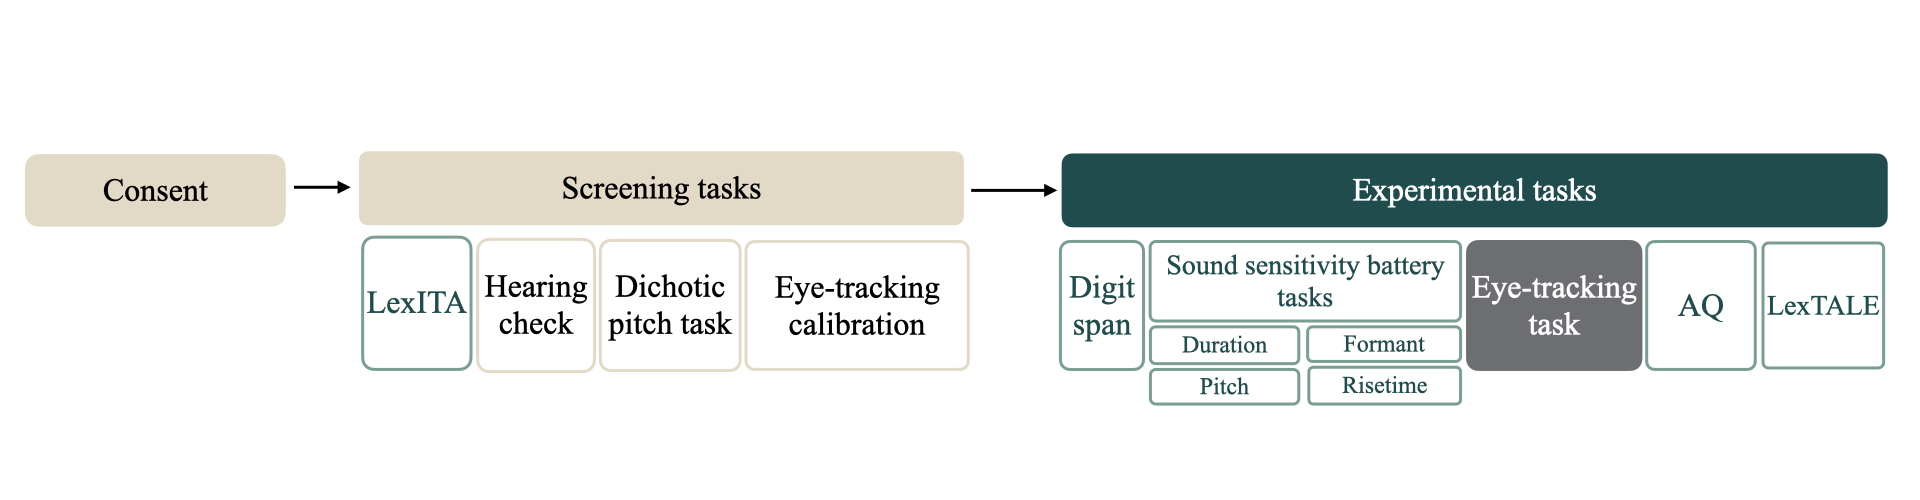
\includegraphics[width=1\linewidth]{visuals/task_structure.jpg} % Adjust the width as needed
  \caption{Task structure: All tasks are ordered from beginning (left) to end (right). Those underneath calibration tasks were used to filter out participants. Those that are in tan were used as measures in our study. Italian Lextale is both a measure and a filter.}
  \label{fig:task_structure}
\end{figure}

After consenting and completing the initial screening tasks, participants began the digit span task. The digit span task presented a series of digits displayed for 500 ms per digit separated by a 250 ms fixation cross. Participants were asked to use their mouse to select the sequence in the same order on a digital number pad. The task began with two digits and had a staircase design with sequence length increasing by one after each correct trial and decreasing by one after each incorrect trial. The task ended after 13 trials. 

The four battery tasks consisted of AX discrimination tasks which tested participants' sensitivity to pitch, rise time, duration, and formant contrasts. For each task, the participant was asked to use the `z' and `m' keys to identify same and different pairs, respectively. For all battery tasks, a continuum of 50 stimuli was used \citep{Krizman_2019}. 10 of these were selected at various distances (15-55). The distance between stimuli and same/different trials was presented randomly.

During the eye-tracking task, all 64 experimental and distractor words were shown in lower-case letters balanced across the four quadrants. Eye-fixations were captured using WebGazer.js \citep{Papoutsaki} implemented in Gorilla \citep{Anwyl-Irvine_2019}. All audio stimuli and word pairings were taken from \cite{Sulpizio_McQueen_2012}. Visual stimuli were placed maximally apart to increase the distance between areas of interest. Distractor and experimental trials were presented in random order. Like \cite{Sulpizio_McQueen_2012}, each trial began with a fixation cross that was displayed for 500 ms. Next, the audio stimuli and visual stimuli were presented simultaneously. After the audio file finished playing ($\mu$ = 110 ms, \textit{sd} = 51 ms), visual stimuli stayed on the screen for 500 ms for the participant to select the word that they had been presented. Before the experiment, \cite{Sulpizio_McQueen_2012} did a read-aloud familiarization task with the participants, but zero words were unknown to any participant. For this reason, we decided to remove the familiarization task due to the consistent low frequency of all auditory stimuli and the previously tested high consistency accuracy.

After completion of the eye-tracking task, participants then took part in an English Lextale task as well as an ASDQ. Both of these tasks were purposefully put after the eye-tracking task to mitigate negative effects on task performance \citep{Chang_2024}. In the English Lextale task, participants were shown a fixation cross for 500 ms and then a word or non-word was displayed for 2000 ms. They then needed to use the keys to decide if the word was a real `j' or not `k' within the allotted time. The Italian Lextale task that was used during calibration was exactly the same as the English Lextale but with Italian words. While the task was used as a filter to ensure participants could speak Italian, scores for both the English and Italian Lextale were used as individual difference measures in the present study.

Lastly, for ASDQ, 50 questions with four selection options were given (i.e., ``strongly disagree", ``disagree", ``agree", and ``strongly agree"). The direction of high tendency scoring was balanced across questions (i.e., ``strongly agree" and ``strongly disagree" were marked as high tendency equally).

\subsection{Data analysis}

The individual difference measures were calculated so that each participant had a single score for each task. For the digit span task, each participant's max digit correct was used as a measure of working memory capacity. For the four battery tasks, hits and misses for each trial were scored and sensitivity to each contrast type was then calculated using d-prime. The Lextale scores for both Italian and English Lextale were calculated by taking the mean of correct and incorrect responses (non-responses were ignored). Lastly, the ASDQ was scored by providing a 1 for answers in the direction of the autistic tendencies and 0 for away (strong agree-agree and strongly disagree-disagree were collapsed). The points were then averaged between questions to calculate an average score.

For eye-tracking data removal, eye-fixations outside the possible screen area were removed. As suggested in \cite{bramlett_wiener_24-AOW}, quadrants were defined by origin to maximize signal retention. Both fixation and frame rate data removal were based on \cite{bramlett_wiener_24-AOW}. Fixations at the beginning of the trials were normally distributed from the center at the beginning trials along both the x and y axes. Eye-fixations with face confirmation below 50\% certainty were removed. We retained approximately 96.14\% of eye-fixations (3.86\% data loss). Unlike other recent online web-based eye-tracking experiments we did not remove any data for low frame rate. We set a minimal frame rate for participants to 5 fps \citep{Vos_2017}. However, no participants qualified for removal based on their median frame rate. 